% mycsrf 'for beeing included' snippet template
%
% (c) Karsten Reincke, Frankfurt a.M. 2012, ff.
%
% This text is licensed under the Creative Commons Attribution 3.0 Germany
% License (http://creativecommons.org/licenses/by/3.0/de/): Feel free to share
% (to copy, distribute and transmit) or to remix (to adapt) it, if you respect
% how you must attribute the work in the manner specified by the author(s):
% \newline
% In an internet based reuse please link the reused parts to mycsrf.fodina.de
% and mention the original author Karsten Reincke in a suitable manner. In a
% paper-like reuse please insert a short hint to mycsrf.fodina.de and to the
% original author, Karsten Reincke, into your preface. For normal quotations
% please use the scientific standard to cite
%


%% use all entries of the bibliography

\subsubsection{ABCJ ($\bigstar$)}

\label{ABCJ}\acc{ABCJ} bezeichnet sich als \enquote{Java Editor, Player und
Bibliothekar für Musikdateien}\footnote{\cite[vgl.][\nopage wp.]{Spencer2019a}.
Im Original: \enquote{a pure-Java editor, player and librarian for music files
stored using Chris Walshaw's ABC notation}}.
\begin{wrapfigure}{r}{6cm}
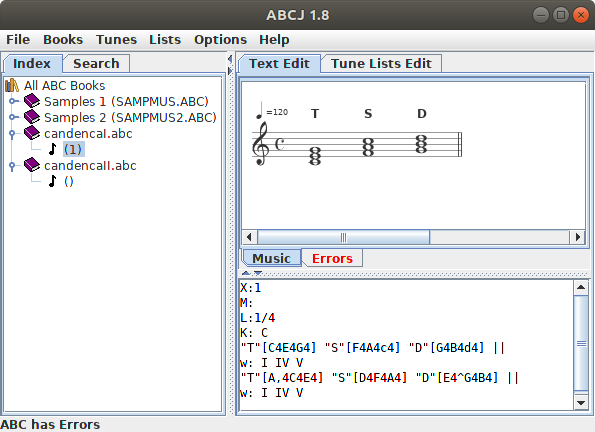
\includegraphics[width=5.5cm]{frontends/abcj/abcj-cadenca1-300dpi.png}
\end{wrapfigure}
Seine herausragende Eigenschaft dürfte sein, dass er \acc{ABC} notierte
Musikstücke in 'Playlisten' erfasst, für deren einzelne Einträge er den
zugehörigen \acc{ABC}-Code editierbar macht und daraus \acc{on the fly} das
entsprechende Notenbild ableitet.

Das Programm wird als JAR-File mit graphischem Installer zum Downoad angeboten;
sofern man die einfachen Vorbedingungen erfüllt hat\footcite[vgl.][\nopage
wp]{Spencer2019a}, läuft die Installation reibungslos durch.

Einige Eigenarten zwingen uns jedoch, an \acc{ABCJ} nur einen Stern zu vergeben:

\begin{itemize}
  \item Zum ersten kann er nicht mit allen Syntagmen umgehen. So vermag er
  unsere Referenzkadenz I, die wir mit dem Konverter \acc{abcm2ps} haben
  erfolreich erzeugen können, nicht vollständig in Noten umzuwandeln, den Code
  unser Referenzkadenz II überhaupt nicht\footnote{Rein logisch gesehen, könnte
  der Fehler auch auf unser Seite liegen. Wir könnten unzulässigen Code genutzt
  haben, den 'unser' Tool \acc{abcm2ps} -- wie auch immer -- noch zu tolerieren
  weiß. Der Effekt ist aber derselbe: \acc{ABCJ} steht nicht ohne
  Zusatzüberlegungen zur Verfügung.}: So bald der ABCJ-Parser das nächste Token
  nicht erkennt, bricht er die Umwandlung ab. Das liegt in der Natur eines
  Parsers. Nicht 'natürlich' ist hingegen, dass er nicht alles, was syntaktisch
  (in \acc{ABC-Plus}) erlaubt ist, auch versteht.
  \item Zum zweiten bietet \acc{ABCJ} als Exportformat nur \acc{ABC}-Code und
  \acc{MIDI} an. Ihn als Brücke in andere Welten zu nutzen, scheidet damit aus.
  \item Der Editor erlaubt gar keine graphische Noteneingabe, sondern ist 'nur'
  ein Texteditor mit angebundener Visualisierung\footnote{Das allein ist kein
  Ausschlusskriterium. Im Gegenteil: wir werden mit \acc{Frescobaldi} und
  \acc{Elysium} zwei andere Frontendsystem vorführen, die dasselbe Konzept
  verfolgen. Allerdings sind deren textuelle Editierfunktionen reicher.}. Die
  Editorfunktionen sind allerdings recht rudimentär, jedenfalls keine
  Code-Completion und kein Syntaxhighlighting.
\end{itemize}

Damit scheidet \acc {ABCJ} für Musikwissenschaftler als Frontend aus. So gerne
wir dem Programm auch mehr Reputation gezollt hätten -- es ist echte freie
Software -- und so erkennbar viel Arbeit sein Autor hineingesteckt hat, so wenig
ist es leider für unsere Zwecke geeignet.


% this is only inserted to eject fault messages in texlipse
%\bibliography{../bib/literature}
